\section{Stato dei requisiti funzionali}

Si riporta ciascun requisito mediante il corrispondente codice,
rispetto alla stessa tabella presente nel documento \textit{Analisi dei Requisiti v2.0.0 - Sez. Req. Funzionali}, qui è presente
una colonna indicante la soddisfazione di tale requisito.

\newcounter{rowcounter}
\setcounter{rowcounter}{0}

\begin{longtable}{|C{1.5cm}|C{2cm}|L{5cm}|C{2cm}|}
    \hline
    \textbf{Codice} & \textbf{Importanza} & \textbf{Descrizione} & \textbf{Stato} \\
    
    %RF1
    \hline
    RF\arabic{rowcounter} & Obbligatorio &
    L'accesso al prodotto è vincolato da un \textit{sistema}\textsubscript{\textit{G}} di \textit{login}\textsubscript{\textit{G}}, tuttavia, non è necessario che gli utenti si registrino autonomamente. Le credenziali di accesso sono fornite da terze parti o dall'amministratore del \textit{sistema}\textsubscript{\textit{G}}.& Soddisfatto \\
    
    %RF2
    \hline
    \stepcounter{rowcounter} RF\arabic{rowcounter} & Obbligatorio & Il prodotto non deve avere una gestione di amministrazione. & Soddisfatto \\
    
    %RF3
    \hline
    \stepcounter{rowcounter} RF\arabic{rowcounter} & Obbligatorio & Il \textit{sistema}\textsubscript{\textit{G}} deve integrare simulatori di diverso tipo al fine di generare dati di misurazioni che siano coerenti con l'ambito del \textit{sensore}\textsubscript{\textit{G}} simulato. & Soddisfatto \\
    
    %RF4
    \hline
    \stepcounter{rowcounter} RF\arabic{rowcounter} & Obbligatorio & Ogni misurazione trasmessa dal simulatore del \textit{sensore}\textsubscript{\textit{G}} deve essere composta dall'id del \textit{sensore}\textsubscript{\textit{G}}, il timestamp e la misurazione. & Soddisfatto\\
    
    %RF5
    \hline
    \stepcounter{rowcounter} RF\arabic{rowcounter} & Obbligatorio &  Il \textit{sistema}\textsubscript{\textit{G}} deve essere in grado di simulare almeno un \textit{sensore}\textsubscript{\textit{G}} che rilevi la temperatura espressa in gradi Celsius.& Soddisfatto \\
    
    %RF6
    \hline
    \stepcounter{rowcounter} RF\arabic{rowcounter} & Obbligatorio &  Il \textit{sistema}\textsubscript{\textit{G}} deve essere in grado di simulare almeno un \textit{sensore}\textsubscript{\textit{G}} che misuri l'umidità, espressa in percentuale di umidità nell'aria. & Soddisfatto \\
    
    %RF7
    \hline
    \stepcounter{rowcounter} RF\arabic{rowcounter} & Obbligatorio &  Il \textit{sistema}\textsubscript{\textit{G}} deve essere in grado di simulare almeno un \textit{sensore}\textsubscript{\textit{G}} per la rilevazione delle particelle di polveri sottili presenti nell'aria, espresse in microgrammi per metro cubo. & Soddisfatto \\
    
    %RF8
    \hline
    \stepcounter{rowcounter} RF\arabic{rowcounter} & Obbligatorio &  Il \textit{sistema}\textsubscript{\textit{G}} deve includere la simulazione di almeno un \textit{sensore}\textsubscript{\textit{G}} per individuare guasti elettrici. Questi sensori segnalano interruzioni nella fornitura di energia elettrica tramite un \textit{bit}\textsubscript{\textit{G}} binario, con il valore 0 che indica l'assenza di energia elettrica. & Soddisfatto \\
    
    %RF9
    \hline
    \stepcounter{rowcounter} RF\arabic{rowcounter} & Obbligatorio &  Il \textit{sistema}\textsubscript{\textit{G}} deve essere in grado di simulare almeno un \textit{sensore}\textsubscript{\textit{G}} per monitorare lo stato di riempimento dei diversi conferitori nelle isole ecologiche. L'indicazione fornita sarà una percentuale di riempimento dell'isola ecologica. & Soddisfatto \\
    
    %RF10
    \hline
    \stepcounter{rowcounter} RF\arabic{rowcounter} & Obbligatorio & Il \textit{sistema}\textsubscript{\textit{G}} deve includere la simulazione di almeno un \textit{sensore}\textsubscript{\textit{G}} per le colonnine di ricarica. Questi sensori indicheranno tramite un \textit{bit}\textsubscript{\textit{G}} binario se la colonnina è occupata (\textit{bit}\textsubscript{\textit{G}} 1) o libera (\textit{bit}\textsubscript{\textit{G}} 0). & Soddisfatto \\
    
    %RF11
    \hline
    \stepcounter{rowcounter} RF\arabic{rowcounter} & Obbligatorio & Il \textit{sistema}\textsubscript{\textit{G}} deve includere la simulazione di almeno un \textit{sensore}\textsubscript{\textit{G}} per il livello dell'acqua. Questi sensori indicheranno il livello dell'acqua.& Soddisfatto \\
    
    %RF12
    \hline
    \stepcounter{rowcounter} RF\arabic{rowcounter} & Obbligatorio &  Ogni dato generato dai simulatori dei sensori deve essere strettamente correlato al dato successivo, garantendo così una transizione realistica e plausibile tra le misurazioni.& Soddisfatto \\
    
    %RF13
    \hline
    \stepcounter{rowcounter} RF\arabic{rowcounter} & Obbligatorio & Il \textit{sistema}\textsubscript{\textit{G}} deve essere in grado di memorizzare in modo sicuro e efficiente i dati generati dai sensori. Ciò include la registrazione accurata di ogni misurazione, assicurando l'integrità e la coerenza dei dati.& Soddisfatto \\
    
    %RF14
    \hline
    \stepcounter{rowcounter} RF\arabic{rowcounter} & Obbligatorio & La \textit{piattaforma}\textsubscript{\textit{G}} deve supportare la visualizzazione di dati provenienti da diversi tipi di sensori.& Soddisfatto \\
    
    %RF15
    \hline
    \stepcounter{rowcounter} RF\arabic{rowcounter} & Obbligatorio & L'utente deve poter visualizzare una \textit{dashboard}\textsubscript{\textit{G}} con una panoramica completa dello stato della città tramite l'utilizzo di \textit{widget}\textsubscript{\textit{G}} adibiti alla rappresentazione delle misurazioni dei sensori.& Soddisfatto \\
    
    %RF16
    \hline
    \stepcounter{rowcounter} RF\arabic{rowcounter} & Obbligatorio & L'utente deve avere la possibilità di visualizzare le misurazioni all'interno dei \textit{widget}\textsubscript{\textit{G}} adibiti alla rappresentazione delle rilevazioni dei sensori in formato grafico time series.& Soddisfatto \\
    
    %RF17
    \hline
    \stepcounter{rowcounter} RF\arabic{rowcounter} & Obbligatorio & L'utente deve avere la possibilità di visualizzare le misurazioni all'interno dei \textit{widget}\textsubscript{\textit{G}} adibiti alla rappresentazione delle rilevazioni dei sensori in formato testuale time series.& Soddisfatto \\
    
    %RF18
    \hline
    \stepcounter{rowcounter} RF\arabic{rowcounter} & Obbligatorio & La visualizzazione delle misurazioni in formato testuale time series deve presentare le informazioni nel formato: \texttt{IDSensore ,TIMESTAMP, Dato}.& Soddisfatto \\
   
    %RF19
    \hline
    \stepcounter{rowcounter} RF\arabic{rowcounter} & Obbligatorio &  L'utente deve essere in grado di visualizzare le ultime misurazioni all'interno dei \textit{widget}\textsubscript{\textit{G}} dedicati alla presentazione dei rilevamenti dei sensori che trasmettono dati binari (ex. Occupato/Libero) attraverso una mappa interattiva. La mappa, tramite etichette adeguate, deve rappresentare chiaramente il valore corrispondente all'ultima misurazione effettuata da ciascun \textit{sensore}\textsubscript{\textit{G}}.& Soddisfatto \\
    
    %RF20
    \hline
    \stepcounter{rowcounter} RF\arabic{rowcounter} & Obbligatorio & La \textit{dashboard}\textsubscript{\textit{G}} richiede un aggiornamento quasi istantaneo per garantire che i dati provenienti dai sensori siano riflessi nel minor tempo possibile, entro un massimo di 10 secondi.& Soddisfatto \\
    
    %RF21
    \hline
    \stepcounter{rowcounter} RF\arabic{rowcounter} & Obbligatorio & La \textit{dashboard}\textsubscript{\textit{G}} deve mostrare un \textit{widget}\textsubscript{\textit{G}} distinto per ciascun tipo di \textit{sensore}\textsubscript{\textit{G}} attivo che trasmette dati al \textit{sistema}\textsubscript{\textit{G}}, contenente le misurazioni in formato grafico, testuale o mappa interattiva.& Soddisfatto \\
    
    %RF22
    \hline
    \stepcounter{rowcounter} RF\arabic{rowcounter} & Obbligatorio & Ogni \textit{widget}\textsubscript{\textit{G}} che visualizza le misurazioni deve includere, insieme ai dati stessi, informazioni sull'identificativo dei sensori che hanno contribuito a quelle misurazioni.& Soddisfatto \\
    
    %RF23
    \hline
    \stepcounter{rowcounter} RF\arabic{rowcounter} & Obbligatorio & La \textit{dashboard}\textsubscript{\textit{G}} deve includere un \textit{widget}\textsubscript{\textit{G}} dedicato alle misurazioni dei sensori di temperatura.& Soddisfatto \\
    
    %RF24
    \hline
    \stepcounter{rowcounter} RF\arabic{rowcounter} & Obbligatorio &Il \textit{widget}\textsubscript{\textit{G}} destinato alla rappresentazione delle misurazioni effettuate dai sensori di temperatura deve offrire all'utente di default la visualizzazione di tali dati in un formato grafico a linee, con una linea corrispondente a ciascun \textit{sensore}\textsubscript{\textit{G}} coinvolto.& Soddisfatto \\
    
    %RF25
    \hline
    \stepcounter{rowcounter} RF\arabic{rowcounter} & Obbligatorio & La \textit{dashboard}\textsubscript{\textit{G}} deve includere un \textit{widget}\textsubscript{\textit{G}} dedicato alle misurazioni dei sensori di umidità.& Soddisfatto \\
    %RF26
    \hline
    \stepcounter{rowcounter} RF\arabic{rowcounter} & Obbligatorio &Il \textit{widget}\textsubscript{\textit{G}} destinato alla rappresentazione delle misurazioni effettuate dai sensori di umidità deve offrire all'utente di default la visualizzazione di tali dati in un formato grafico a linee, con una linea corrispondente a ciascun \textit{sensore}\textsubscript{\textit{G}} coinvolto.& Soddisfatto \\
    
    %RF27
    \hline
    \stepcounter{rowcounter} RF\arabic{rowcounter} & Obbligatorio & La \textit{dashboard}\textsubscript{\textit{G}} deve includere un \textit{widget}\textsubscript{\textit{G}} dedicato alle misurazioni dei sensori delle polveri sottili.& Soddisfatto \\
    
    %RF28
    \hline
    \stepcounter{rowcounter} RF\arabic{rowcounter} & Obbligatorio &Il \textit{widget}\textsubscript{\textit{G}} destinato alla rappresentazione temporale delle misurazioni effettuate dai sensori di polveri sottili deve offrire all'utente la possibilità di visualizzare tali dati in un formato grafico a linee, con una linea corrispondente a ciascun \textit{sensore}\textsubscript{\textit{G}} coinvolto.& Soddisfatto \\
    
    %RF29
    \hline
    \stepcounter{rowcounter} RF\arabic{rowcounter} & Obbligatorio & La \textit{dashboard}\textsubscript{\textit{G}} deve includere un \textit{widget}\textsubscript{\textit{G}} dedicato alle misurazioni dei sensori dei guasti elettrici.& Soddisfatto \\
    
    %RF30
    \hline
    \stepcounter{rowcounter} RF\arabic{rowcounter} & Obbligatorio &Il \textit{widget}\textsubscript{\textit{G}} destinato alla rappresentazione delle misurazioni effettuate dai sensori dei guasti elettrici deve offrire all'utente di default la visualizzazione di tali dati con una mappa interattiva delle ultime misurazioni.  & Soddisfatto \\
    
    %RF31
    \hline
    \stepcounter{rowcounter} RF\arabic{rowcounter} & Obbligatorio & La \textit{dashboard}\textsubscript{\textit{G}} deve includere un \textit{widget}\textsubscript{\textit{G}} dedicato alle misurazioni dei sensori di soglia delle isole ecologiche.& Soddisfatto \\
    
    %RF32
    \hline
    \stepcounter{rowcounter} RF\arabic{rowcounter} & Obbligatorio &Il \textit{widget}\textsubscript{\textit{G}} destinato alla rappresentazione delle misurazioni effettuate dai sensori di soglia delle isole ecologiche deve offrire all'utente la visualizzazione di tali dati con una mappa interattiva delle ultime misurazioni.  & Soddisfatto \\
    
    %RF33
    \hline
    \stepcounter{rowcounter} RF\arabic{rowcounter} & Obbligatorio & La \textit{dashboard}\textsubscript{\textit{G}} deve includere un \textit{widget}\textsubscript{\textit{G}} dedicato alle misurazioni dei sensori delle colonnine di ricarica. & Soddisfatto \\
    
    %RF34
    \hline
    \stepcounter{rowcounter} RF\arabic{rowcounter} & Obbligatorio &Il \textit{widget}\textsubscript{\textit{G}} destinato alla rappresentazione delle misurazioni effettuate dai sensori delle colonnine di ricarica deve offrire all'utente la visualizzazione di tali dati con una mappa interattiva delle ultime misurazioni.  & Soddisfatto \\
    
    %RF35
    \hline
    \stepcounter{rowcounter} RF\arabic{rowcounter} & Obbligatorio & La \textit{dashboard}\textsubscript{\textit{G}} deve includere un \textit{widget}\textsubscript{\textit{G}} dedicato alle misurazioni dei sensori del livello dell'acqua. & Soddisfatto \\
    
    %RF36
    \hline
    \stepcounter{rowcounter} RF\arabic{rowcounter} & Obbligatorio &Il \textit{widget}\textsubscript{\textit{G}} destinato alla rappresentazione delle misurazioni effettuate dai sensori del livello dell'acqua deve offrire all'utente la visualizzazione di tali dati con una mappa interattiva delle ultime misurazioni. & Soddisfatto \\
    
    %RF37
    \hline
    \stepcounter{rowcounter} RF\arabic{rowcounter} & Obbligatorio & La \textit{dashboard}\textsubscript{\textit{G}} della città deve includere una mappa interattiva che mostra la posizione dei diversi sensori nella città.& Soddisfatto \\
    
    %RF38
    \hline
    \stepcounter{rowcounter} RF\arabic{rowcounter} & Obbligatorio & I sensori nella mappa devono essere etichettati in modo da consentirne il riconoscimento della tipologia.& Soddisfatto \\
    
    %RF39
    \hline
    \stepcounter{rowcounter} RF\arabic{rowcounter} & Obbligatorio &  I sensori posizionati sulla mappa devono visualizzare l'ultimo valore registrato quando il puntatore del mouse è posizionato sopra di essi.& Soddisfatto \\
    
    %RF40
    \hline
    \stepcounter{rowcounter} RF\arabic{rowcounter} & Desiderabile & La \textit{dashboard}\textsubscript{\textit{G}} deve fornire un \textit{widget}\textsubscript{\textit{G}} con il punteggio di salute relativo alla città basato sui dati aggregati provenienti dai sensori.& Soddisfatto \\
    
    %RF41
    \hline
    \stepcounter{rowcounter} RF\arabic{rowcounter} & Obbligatorio & L'utente deve avere la possibilità di selezionare una cella, ovvero un'area specifica della città, al fine di visualizzare una \textit{dashboard}\textsubscript{\textit{G}} dedicata contenente esclusivamente sensori, misurazioni e punteggio di salute correlati a essa.& Soddisfatto \\
    
    %RF42
    \hline
    \stepcounter{rowcounter} RF\arabic{rowcounter} & Obbligatorio & L'utente deve poter filtrare la visualizzazione delle misurazioni di una specifica tipologia di sensori inserendo uno specifico intervallo temporale.& Soddisfatto \\
    
    %RF43
    \hline
    \stepcounter{rowcounter} RF\arabic{rowcounter} & Obbligatorio & Il \textit{sistema}\textsubscript{\textit{G}} deve verificare la validità dell'intervallo temporale inserito dall'utente.& Soddisfatto \\
    
    %RF44
    \hline
    \stepcounter{rowcounter} RF\arabic{rowcounter} & Obbligatorio & In caso di intervallo temporale non valido, il \textit{sistema}\textsubscript{\textit{G}} deve generare una notifica di errore.& Soddisfatto \\
    
    %RF45
    \hline
    \stepcounter{rowcounter} RF\arabic{rowcounter} & Obbligatorio & La notifica di errore relativa all'inserimento di un intervallo temporale non valido deve richiedere all'utente di reinserire date valide.& Soddisfatto \\
    
    %RF46
    \hline
    \stepcounter{rowcounter} RF\arabic{rowcounter} & Obbligatorio & La notifica di errore relativa all'inserimento di un intervallo temporale non valido deve essere chiara e informativa, indicando il motivo specifico dell'invalidità dell'intervallo temporale (data fine precedente a data inizio, arco temporale precedente o antecedente all'inizio della trasmissione dati).& Soddisfatto \\
    
    %RF47
    \hline
    \stepcounter{rowcounter} RF\arabic{rowcounter} & Obbligatorio & L'utente ha la possibilità di selezionare l'intervallo temporale desiderato (secondo, minuto, ora, giorno, mese, anno) per aggregare le misurazioni in base al relativo periodo di registrazione corrispondente.& Soddisfatto \\
    
    %RF48
    \hline
    \stepcounter{rowcounter} RF\arabic{rowcounter} & Obbligatorio & Il \textit{sistema}\textsubscript{\textit{G}} deve essere in grado di adattare dinamicamente la rappresentazione delle misurazioni secondo un intervallo temporale di aggregazione selezionato dall'utente.& Soddisfatto \\
    
    %RF49
    \hline
    \stepcounter{rowcounter} RF\arabic{rowcounter} & Obbligatorio &  L'utente deve avere la possibilità di definire due valori (un minimo e un massimo) per filtrare le misurazioni dei sensori di una specifica tipologia, utilizzando questi limiti come criterio per visualizzare solo i dati compresi in quei range.& Soddisfatto \\
    
    %RF50
    \hline
    \stepcounter{rowcounter} RF\arabic{rowcounter} & Obbligatorio & Il \textit{sistema}\textsubscript{\textit{G}} deve verificare la validità dell'intervallo di rilevamento inserito dall'utente.& Soddisfatto \\
    
    %RF51
    \hline
    \stepcounter{rowcounter} RF\arabic{rowcounter} & Obbligatorio & In caso di intervallo di rilevamento non valido, il \textit{sistema}\textsubscript{\textit{G}} deve generare una notifica di errore.& Soddisfatto \\
    
    %RF52
    \hline
    \stepcounter{rowcounter} RF\arabic{rowcounter} & Obbligatorio & La notifica di errore relativa all'inserimento di un intervallo di rilevamento non valido deve richiedere all'utente di reinserire valori validi.& Soddisfatto \\
    
    %RF53
    \hline
    \stepcounter{rowcounter} RF\arabic{rowcounter} & Obbligatorio & La notifica di errore relativa all'inserimento di un intervallo di rilevamento non valido deve essere chiara e informativa, indicando il motivo specifico dell'invalidità dell'intervallo di rilevamento (data fine precedente a data inizio, arco temporale precedente o antecedente all'inizio della trasmissione dati).& Soddisfatto \\
    
    %RF54
    \hline
    \stepcounter{rowcounter} RF\arabic{rowcounter} & Obbligatorio & L'utente deve avere la possibilità di filtrare le misurazioni selezionando uno o più sensori di una specifica categoria in modo tale da visualizzare esclusivamente le misurazioni corrispondenti ai sensori selezionati.& Soddisfatto \\
    
    %RF55
    \hline
    \stepcounter{rowcounter} RF\arabic{rowcounter} & Obbligatorio & L'utente deve poter filtrare la visualizzazione delle misurazioni di una specifica tipologia di sensori selezionando una o più specifiche celle come criterio di filtro.& Soddisfatto \\
    
    %RF56
    \hline
    \stepcounter{rowcounter} RF\arabic{rowcounter} & Obbligatorio & L'utente deve poter applicare più filtri simultaneamente per la visualizzazione delle misurazioni di una specifica tipologia di sensori.& Soddisfatto \\
    
    %RF57
    \hline
    \stepcounter{rowcounter} RF\arabic{rowcounter} & Obbligatorio & L'utente deve poter rimuovere i filtri applicati e ripristinare la visualizzazione senza tali filtri.& Soddisfatto \\

    %RF58
    \hline
    \stepcounter{rowcounter} RF\arabic{rowcounter} & Opzionale & L'utente deve poter salvare in una lista di misurazioni rilevanti una misurazione trasmessa da un \textit{sensore}\textsubscript{\textit{G}}.& Non soddisfatto \\
    
    %RF59
    \hline
    \stepcounter{rowcounter} RF\arabic{rowcounter} & Opzionale & Il \textit{sistema}\textsubscript{\textit{G}} deve effettuare una verifica prima di salvare la misurazione tra le misurazioni rilevanti, assicurandosi che il dato non sia già presente in tale lista.& Non soddisfatto \\
    
    %RF60
    \hline
    \stepcounter{rowcounter} RF\arabic{rowcounter} & Opzionale & L'utente deve poter visualizzare la lista delle misurazioni rilevanti.& Non soddisfatto \\
    
    %RF61
    \hline
    \stepcounter{rowcounter} RF\arabic{rowcounter} & Opzionale & Ogni misurazione nella lista dei rilevanti deve fornire l'identificativo del \textit{sensore}\textsubscript{\textit{G}} che ha effettuato la misurazione.& Non soddisfatto \\

    %RF62
    \hline
    \stepcounter{rowcounter} RF\arabic{rowcounter} & Opzionale & Ogni misurazione nella lista dei rilevanti deve fornire la tipologia del \textit{sensore}\textsubscript{\textit{G}} che ha effettuato la misurazione.& Non soddisfatto \\

    %RF63
    \hline
    \stepcounter{rowcounter} RF\arabic{rowcounter} & Opzionale & Ogni misurazione nella lista dei rilevanti deve fornire l'orario e la data di misurazione.& Non soddisfatto \\

    %RF64
    \hline
    \stepcounter{rowcounter} RF\arabic{rowcounter} & Opzionale & Ogni misurazione nella lista dei rilevanti deve fornire il valore misurato e la relativa unità di misura.& Non soddisfatto \\

    %RF65
    \hline
    \stepcounter{rowcounter} RF\arabic{rowcounter} & Opzionale & L'utente deve poter rimuovere una misurazione dalla lista delle misurazioni rilevanti.& Non soddisfatto \\

    %RF66
    \hline
    \stepcounter{rowcounter} RF\arabic{rowcounter} & Obbligatorio & L'utente deve essere in grado di ricevere notifiche nel caso in cui i sensori superino determinate soglie di sicurezza.& Soddisfatto \\

    %RF67
    \hline
    \stepcounter{rowcounter} RF\arabic{rowcounter} & Obbligatorio & L'utente deve essere in grado di visualizzare le informazioni dei sensori.& Soddisfatto \\

    %RF68
    \hline
    \stepcounter{rowcounter} RF\arabic{rowcounter} & Obbligatorio & L'utente deve essere in grado di visualizzare l'\textit{ID}\textsubscript{\textit{G}} dei sensori.& Soddisfatto \\

    %RF69
    \hline
    \stepcounter{rowcounter} RF\arabic{rowcounter} & Obbligatorio & L'utente deve essere in grado di visualizzare il tipo dei sensori.& Soddisfatto \\

    %RF70
    \hline
    \stepcounter{rowcounter} RF\arabic{rowcounter} & Obbligatorio & L'utente deve essere in grado di visualizzare la posizione dei sensori in coordinate.& Soddisfatto \\

    %RF71
    \hline
    \stepcounter{rowcounter} RF\arabic{rowcounter} & Obbligatorio & L'utente deve essere in grado di visualizzare la cella in cui è installato il \textit{sensore}\textsubscript{\textit{G}}.& Soddisfatto \\

    %RF72
    \hline
    \stepcounter{rowcounter} RF\arabic{rowcounter} & Obbligatorio & L'utente deve essere in grado di visualizzare la data di installazione dei sensori.& Soddisfatto \\

    %RF73
    \hline
    \stepcounter{rowcounter} RF\arabic{rowcounter} & Obbligatorio & L'utente deve essere in grado di visualizzare l'unità di misura associata al \textit{sensore}\textsubscript{\textit{G}}.& Soddisfatto \\
    
    \hline
    \stepcounter{rowcounter} RF\arabic{rowcounter} & Obbligatorio & La \textit{piattaforma}\textsubscript{\textit{G}} deve poter ricevere più rilevazioni in parallelo. & Soddisfatto \\

    \hline
    
\end{longtable}

\subsection{Grafici riassuntivi requisiti soddisfatti}

\begin{figure}[H]
    \centering
    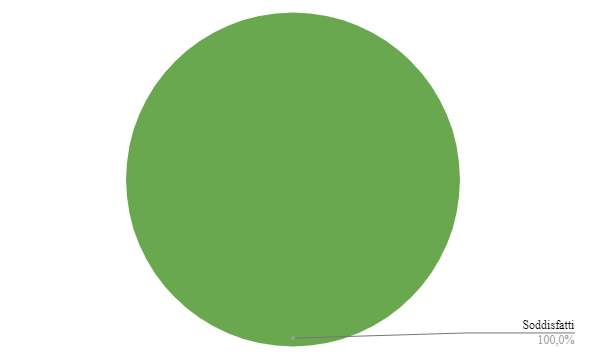
\includegraphics[width=1\textwidth]{../Images/SpecificaTecnica/req_obbligatori.PNG}
    \caption{Stato dei requisiti funzionali obbligatori}
    \label{fig: reqob}
\end{figure}

\begin{figure}[H]
    \centering
    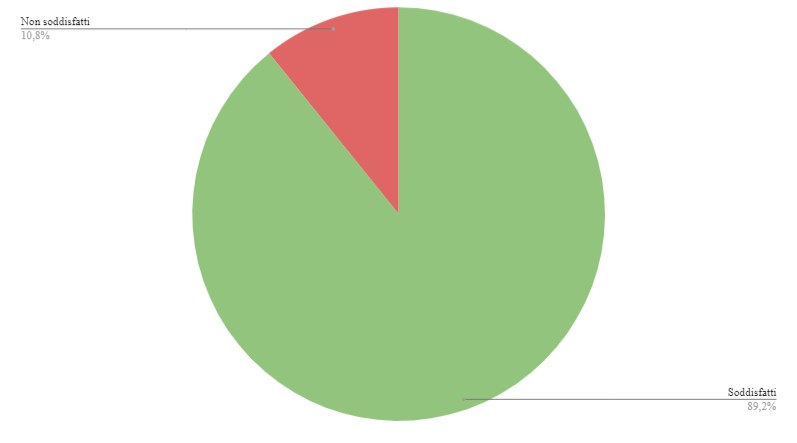
\includegraphics[width=1\textwidth]{../Images/SpecificaTecnica/reqfunz.jpg}
    \caption{Stato dei requisiti funzionali totali}
    \label{fig: reqtot}
\end{figure}